\documentclass[11pt,letterpaper]{article}
\usepackage{graphicx, geometry, amsmath, hyperref, url, booktabs, xcolor, longtable, tabularx, float}
\geometry{margin=1in}
\hypersetup{colorlinks=true, linkcolor=black, citecolor=black, urlcolor=black}
\usepackage[T1]{fontenc}
\usepackage[utf8]{inputenc}

\newcolumntype{L}[1]{>{\raggedright\arraybackslash}p{#1}}
\newcolumntype{C}[1]{>{\centering\arraybackslash}p{#1}}

\title{Open Neighbourhoods Precede Concept Spread:\\Structural Antecedents and Cross-Disciplinary Diffusion\\of Emerging Scientific Concepts\\[1em]\large Internal Research Report}
\author{}
\date{September 2026}

\tolerance=1500
\emergencystretch=1em

\begin{document}
\maketitle
\tableofcontents
\clearpage

%% ============================================================
\section{Overview}
%% ============================================================

This report documents an investigation of how emerging scientific concepts can be identified and characterised through evolving knowledge networks, and through which structural pathways they spread across disciplinary boundaries. The study builds on an OpenAlex-based scholarly dataset of 426 semantically grounded concepts with 462,812 works, constructs yearly co-occurrence and concept-discipline networks, and tests whether structural indicators provide early signals of emergence and cross-disciplinary integration.

Two research questions structure the work.
\textbf{RQ1} asks which temporal and structural patterns in an evolving, semantically grounded scientific knowledge graph characterise the emergence of scientific concepts.
\textbf{RQ2} asks how emerging scientific concepts diffuse across disciplinary communities over time, and which temporal network patterns distinguish locally concentrated concepts from concepts that become broadly integrated into the scientific knowledge network.

The study began with a source-sink viability hypothesis adapted from population ecology, asking whether a concept's presence in a subfield is self-sustaining or import-dependent. That hypothesis was blocked by insufficient citation-layer density (Gate~A failure: only 17.3\% of edges meet the within-host tracing threshold), triggering a pre-registered fallback.

For the emergence question (RQ1), the primary closure measure did not survive held-out confirmation (R1\_DEAD under the frozen kill rule: Holm $p = 0.147$). Only persistent-neighbour closure is confirmed (held-out $S = -1.07$, Holm $p = 0.015$). The effect is not Burt brokerage (constraint is higher, not lower).

For the diffusion question (RQ2), when a concept enters a new host subfield, the share of its initial co-occurrence partners that are native to that host predicts subsequent uptake by newcomer authors (held-out co-primary IRR/SD 1.19 [1.06, 1.33], $p = 0.004$, MeSH replication IRR/SD 1.23 [1.12, 1.36], Holm $p < 0.001$), while co-transfer of origin companions is null.

The target venue is Applied Network Science.

%% ============================================================
\section{Iteration 1: Data Foundation and Pre-Registration}
\label{sec:iter1}
%% ============================================================

\subsection{Strategy}

The first iteration was devoted to three preparatory tasks: (a)~assembling a prior-art and pre-registration dossier grading each candidate mechanism's novelty and feasibility, (b)~building the concept pool and its associated OpenAlex work corpus, and (c)~constructing the semantic grounding infrastructure (concept detection, labelling, variant merging) and a held-out MeSH confirmation population. No experiment or evaluation was executed. Every artifact in this iteration is either a dataset or a research dossier. The rationale was to fix all operational definitions, sample the data, and verify the citation-layer gate (Gate~A) before committing compute to network construction and statistical modelling.

The pre-registration dossier ranks five candidate mechanisms by novelty margin against the nearest prior work. Host anchoring (the share of a concept's new co-occurrence edges in a host subfield that attach to host-native concepts) was ranked highest at medium-to-high novelty; toolkit co-transfer (the fraction of a concept's origin companions that co-appear in host papers) was ranked high on measurement novelty but coupled to host anchoring; citation-lineage source-sink viability was ranked medium. Origin-neighbourhood structure was ranked low-to-medium because structural diversity and community spread are well studied, and the demic-versus-cultural adoption channel was ranked medium but with the weakest feasibility due to author-disambiguation biases.

A pre-registered screen was fixed before any data were inspected. The unit of analysis is a concept~$c$ in non-origin subfield~$d$ at focal year~$t$ (2010--2014), with at least 10 $d$-papers in $W_1 = [t{-}5, t]$. The primary measure is out-of-sample ROC-AUC for establishment in $W_2 = [t{+}1, t{+}5]$, where establishment means at least 5 $W_2$ $d$-papers by author-disjoint newcomers and presence in at least 3 of the 5 $W_2$ years. Each candidate adds only its own pre-registered scores. A candidate survives if its delta-AUC over BASE has a concept-bootstrap (1,000~reps) 95\%~CI lower bound above~0, its point gain is at least 0.01, and the coefficient sign matches its prediction.

\subsection{Artifact 1: Concept Pool and OpenAlex Work Corpus (gen\_art\_dataset\_1)}

The concept pool was built in an outcome-blind frame. The sample was frozen and hashed before any post-appearance-window data were inspected. The pool comprises 206 concepts, of which 184 are main emerging concepts (first appearance year~$F$ in 2005--2016, with 20--300 papers in the window $F$ to $F{+}2$ and no more than 8,000 total works through 2024) and 22 stationary reference concepts. The 184 main concepts are split by a deterministic hash into a screen fold of 123 and a held-out concept fold of~61; focal-year tags are separate (screen 2010--2014, held-out 2016--2018).

The pool is heavily dominated by arXiv-sourced concepts. Of 366 eligible candidates, 363 came from the arXiv-mined arm, and the final 184 span three origin fields.

\begin{table}[!htbp]
\centering
\caption{Concept pool composition by origin field (Iteration~1, gen\_art\_dataset\_1).}
\label{tab:pool_origin}
\begin{tabular}{lrr}
\toprule
Origin field & Main concepts & Share \\
\midrule
Physics and Astronomy & 82 & 44.6\% \\
Physical Sciences (other) & 56 & 30.4\% \\
Computer Science & 45 & 24.5\% \\
Other & 1 & 0.5\% \\
\midrule
\textbf{Total main} & \textbf{184} & \textbf{100\%} \\
\bottomrule
\end{tabular}
\end{table}

\begin{table}[!htbp]
\centering
\caption{Concept pool by first-appearance band (Iteration~1, gen\_art\_dataset\_1).}
\label{tab:pool_fband}
\begin{tabular}{lr}
\toprule
$F$ band & Count \\
\midrule
2005--2007 & 38 \\
2008--2011 & 76 \\
2012--2016 & 70 \\
\midrule
\textbf{Total} & \textbf{184} \\
\bottomrule
\end{tabular}
\end{table}

Verified links pairing each concept with the OpenAlex works that use it total 214,798 pairs spanning 208,374 unique works. Among the 121,829 main-arm links, 56,997 matched in the work title, 51,966 in the abstract, 10,177 through Semantic Scholar only, and 2,689 through OpenAlex concept indexing alone. \emph{[Correction, Iteration~2: the match-evidence counts above are main-arm only; across all 214,798 links the counts are oa\_abstract 98,192, oa\_title 92,043, s2\_only 21,509, oa\_index\_only 3,054.]} Of the 184 main concepts, 24 were discovered natively in OpenAlex and 160 were discovered through the Semantic Scholar index and mapped to OpenAlex (mapping rate~0.93). Twenty-one concepts carry a sense-check failure flag.

\begin{figure}[!htbp]
\centering
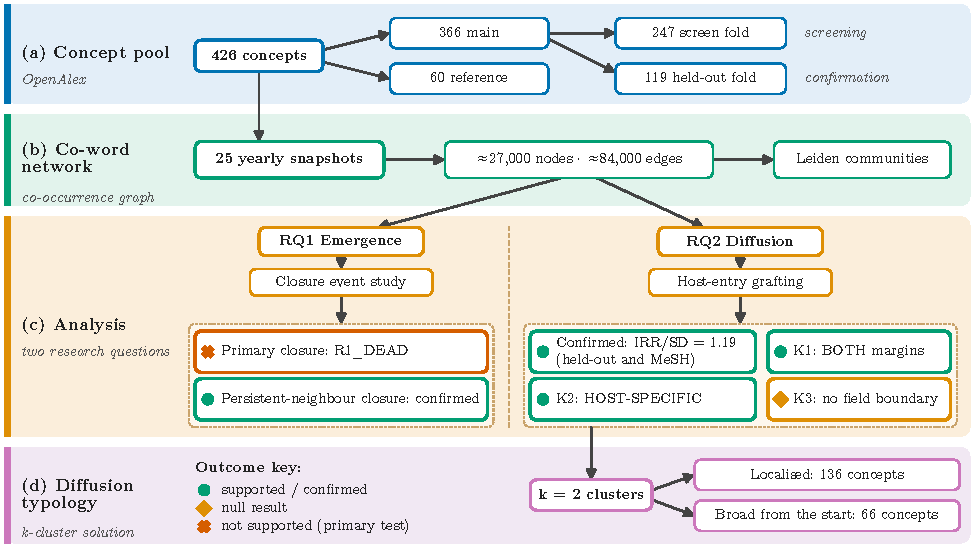
\includegraphics[width=\linewidth,height=0.85\textheight,keepaspectratio]{figures/fig_methodology_v0.pdf}
\caption{Overview of the study design, drawn as four bands linked by arrows. (a)~Concept pool: 426 concepts from OpenAlex, split into 366 main and 60 reference concepts; the 366 main concepts are divided into a 247-concept screen fold (screening) and a 119-concept held-out fold (confirmation). (b)~Co-word network: 25 yearly co-occurrence snapshots ($\approx$27,000 nodes, $\approx$84,000 edges) partitioned into Leiden communities. (c)~Analysis: RQ1 (emergence) tests structural precursors with a closure event study. The primary closure test returns R1\_DEAD, while persistent-neighbour closure is confirmed. RQ2 (diffusion) tests host-entry grafting, which is confirmed (IRR/SD $=1.19$, on the held-out fold and MeSH). Its sub-hypotheses K1 (BOTH margins) and K2 (HOST-SPECIFIC) are supported, and K3 finds no field boundary. (d)~Diffusion typology: a $k=2$ solution separating localised concepts (136) from concepts broad from the start (66).}
\label{fig:methodology}
\end{figure}

\subsubsection{Gate~A: Citation-Layer Feasibility}

The quality report shows that among main-arm concept papers with references, 66.99\% cite at least one earlier concept paper (the ``traced share''), and after excluding first-year canonical papers and the five most-cited concept papers, the traced share remains 60.80\%. The host-specific traced share (concept papers outside the origin subfield that cite at least one earlier concept paper from any subfield, not restricted to the same host subfield) is 55.18\%, above the 40\% gate threshold on the lenient definition. \emph{[Correction, Iteration~2: the original description stated ``at least one earlier concept paper in the same host subfield'', but the code counts any earlier concept paper as a parent regardless of subfield. By year, the lenient host traced share ranges from 0.317 (2010) to 0.517 (2014) across the screen's focal years, with three of five below 0.40. This distinction matters because the within-host share, computed in Iteration~2, is much lower (mean 0.20 on 724 edges), which is the finding that blocks the viability decomposition.]}

\begin{table}[!htbp]
\centering
\caption{Citation-layer quality by origin field (Iteration~1, gen\_art\_dataset\_1).}
\label{tab:cite_quality}
{\small
\begin{tabular}{L{3.2cm}rrrr}
\toprule
Metric & All main & Phys./Astro & Phys.\ Sci & Comp.\ Sci \\
\midrule
Concept papers ($n$) & 121,829 & 19,653 & 46,575 & 55,274 \\
Share w/ references & 83.92\% & 82.04\% & 84.99\% & 83.74\% \\
Traced share (any parent) & 66.99\% & 66.12\% & 67.89\% & 66.53\% \\
Traced (excl.\ $F$ + top-5) & 60.80\% & 57.74\% & 61.75\% & 61.09\% \\
Host traced (any, excl.\ $F$) & 55.18\% & 49.68\% & 58.39\% & 53.86\% \\
Host papers ($n$) & 41,861 & 4,171 & 15,973 & 21,609 \\
\bottomrule
\end{tabular}
}
\end{table}

The recall audit, comparing counts derived from OpenAlex against independent Semantic Scholar counts for 30 concepts, gives a median count ratio of 0.84 (IQR 0.79--0.89) and a Spearman rank correlation of 0.976.

\subsection{Artifact 2: Whole-Science Background Sample (gen\_art\_dataset\_2)}

A design-weighted background sample of 259,716 OpenAlex works from 1,260 strata (150 per field $\times$ year, weights summing to 149,116,575) was built to supply co-occurrence network snapshots and calibrate host-nativeness profiles. It delivered 6,325 exact subfield $\times$ year totals and 400 exact concept $\times$ block subfield profiles for 100 calibration concepts at a cost of \$0.1952 in OpenAlex credits.

The key finding of this artifact is negative: sample-based per-concept subfield profiles are unreliable for determining host-nativeness. In the calibration table, the median total-variation distance between sample and exact profiles is 0.41--0.79 by frequency decile, and top-subfield agreement is only 0.28--0.65. About 12\% of the weighted frame carries the default low-confidence topic T14423, and concept ancestors are no longer served by the API. The worker timed out after writing all outputs, so its status is ``failed'' while its data are usable.

\subsection{Artifact 3: Held-Out MeSH Confirmation Population (gen\_art\_dataset\_3)}

A separate biomedical confirmation arm was built from new MeSH descriptors (DateEstablished 2006--2016, widened to 2004--2005 and 2017--2018). Starting from 28,472 descriptors, the pipeline selects 5,201 topical descriptors, retains 3,430 after the provenance filter, narrows to 283 passing the PubMed novelty pre-screen and early-volume rule, and adds widening-pool candidates. After the final rule, 191 concepts survive: 99 core 2006--2016, 14 from the 2004--2005 widening, and 78 from the 2017--2018 widening.

\begin{table}[!htbp]
\centering
\caption{MeSH held-out population by branch group (Iteration~1, gen\_art\_dataset\_3).}
\label{tab:mesh_branch}
\begin{tabular}{lr}
\toprule
MeSH branch group & Count \\
\midrule
D (Chemicals and drugs) & 62 \\
A+B (Anatomy, Organisms) & 47 \\
E (Analytical, diagnostic, therapeutic) & 32 \\
C (Diseases) & 22 \\
F+H--N (Psychiatry, Health services, misc.) & 17 \\
G (Phenomena and processes) & 11 \\
\midrule
\textbf{Total} & \textbf{191} \\
\bottomrule
\end{tabular}
\end{table}

Caveats: only approximately 25\% of new MeSH descriptors are genuinely new concepts (the remainder are reclassifications or splits), making MeSH a weak ground truth. Only 13 of 191 have their full non-PubMed works paged; the remaining 178 have PubMed-indexed works only.

\subsection{Artifact 4: Semantic Grounding Infrastructure (gen\_art\_dataset\_4)}

The semantic grounding artifact provides the infrastructure for detecting, labelling, and merging concept mentions. It comprises seven datasets: a stratified corpus of 93,600 English OpenAlex articles with abstracts, 4,599 candidate phrases labelled by two LLMs with an adjudicator, a survivorship-free phrase pool, and ancillary data.

\begin{table}[!htbp]
\centering
\caption{Labelling quality (Iteration~1, gen\_art\_dataset\_4).}
\label{tab:labelling_quality}
\begin{tabular}{L{7cm}r}
\toprule
Metric & Value \\
\midrule
Model A vs model B inter-rater kappa (4-class) & 0.259 \\
Model A vs model B binary kappa (concept vs rest) & 0.267 \\
A vs adjudicator kappa (4-class, silver-gold 200) & 0.632 \\
A vs human anchors binary kappa (SemEval/SciERC) & 0.56 \\
A precision (concept, human-anchored) & 0.79 \\
A recall (concept, human-anchored) & 0.76 \\
\bottomrule
\end{tabular}
\end{table}

The survivorship-free phrase pool yielded only 1 strict-eligible anchored phrase, far below the target of 150.

\subsection{Artifact 5: Prior-Art Dossier and Pre-Registration (gen\_art\_research\_1)}

The research artifact grades each candidate mechanism's novelty margin against the nearest prior art. The headline finding is that the space is active but no prior study estimates a within-host reproduction ratio with an import share per concept-subfield edge, nor tests host anchoring at the edge level.

\begin{table}[!htbp]
\centering
\caption{Candidate mechanism novelty grades (Iteration~1, gen\_art\_research\_1).}
\label{tab:novelty_grades}
\begin{tabular}{L{3.5cm}L{2.5cm}L{5cm}}
\toprule
Candidate & Novelty grade & Nearest prior art \\
\midrule
C1: Host anchoring & Medium-to-high & Cheng et al.\ 2023 \\
C2: Toolkit co-transfer & High (coupled to C1) & No quantitative co-arrival test found \\
C0: Source-sink viability & Medium & Kuhn et al.\ 2014; Maillart et al.\ 2026 \\
C4: Demic vs cultural & Medium & Fontaine et al.\ 2024 \\
C3: Origin-neighbourhood structure & Low-to-medium & Structural diversity literature \\
\bottomrule
\end{tabular}
\end{table}

\subsection{Dead Ends and Shortfalls (Iteration~1)}

\begin{enumerate}
\item \textbf{Concept pool size.} 184 of 400 target concepts realised. The binding constraint was the free-singleton retrieval rate (${\sim}$14 works/s) combined with heavy-tailed concept sizes, after credits were consumed by sibling artifacts sharing one key.
\item \textbf{Field coverage.} The pool draws overwhelmingly from physics, physical sciences, and computer science (363 of 366 eligible candidates from the arXiv-mined arm).
\item \textbf{Survivorship-free phrase pool yield.} 1 of 150 target strict-eligible anchored concepts.
\item \textbf{Labelling quality.} Silver labels only (no human check).
\end{enumerate}

\subsection{What Was Learned}

Iteration~1 established the data foundation and pre-registration. The concept pool of 184 main emerging concepts and 22 reference concepts, with 214,798 verified concept-to-work links and 208,374 unique works, passes the citation-layer gate on the lenient (any-parent) definition but has not been tested at the within-host edge level required for viability estimation. No experiment was executed. No quantitative result about the hypothesis exists.

%% ============================================================
\section{Iteration 2: First Experiments and Gate~A Failure}
\label{sec:iter2}
%% ============================================================

\subsection{Strategy}

Iteration~2 was a FIX iteration with five goals: (i)~complete the hydration and add exact nativeness profiles and a citation-independent venue habitat; (ii)~train and evaluate the concept grounding pipeline; (iii)~compute Gate~A as written (within-host, non-canonical, per $W_1$ year) and estimate viability states; (iv)~build the yearly concept-concept co-occurrence network and run the RQ1 event study; (v)~replicate the RQ1 event study on the MeSH population.

Pre-fixed decision rules for Iteration~3: (a)~if Gate~A FAILS, H1/H2 run with graft labels from the exact nativeness profiles; (b)~H1 is declared a pilot if fewer than ${\sim}$150 concepts carry a tested edge; (c)~RQ1 counts as CONFIRMED only if at least one pre-named precursor has an event-study CI excluding~0 AND a delta-AUC CI excluding~0 on the main screen fold, keeps its sign on MeSH, and holds on the sealed held-out fold; (d)~the held-out fold, the 2016--2018 focal years and the phrase pool remain untouched.

\subsection{Artifact 6: Hydrated Corpus and Nativeness Profiles (gen\_art\_dataset\_5)}

This artifact completes the hydration of the concept pool from 184 to 426 concepts (366 main: screen 247, held-out 119; 60 reference), with 462,812 works and 488,078 verified concept-work links. The frame hash was verified against the frozen sample.

\begin{table}[!htbp]
\centering
\caption{Dataset~6 summary (Iteration~2, gen\_art\_dataset\_5).}
\label{tab:dataset6}
\begin{tabular}{lr}
\toprule
Metric & Value \\
\midrule
Concepts hydrated & 426/426 \\
Works & 462,812 \\
Concept-work links & 488,078 \\
API credits consumed & 7,237 \\
Nativeness profiles & 5,488 (1,372 nodes $\times$ 4 blocks) \\
Host weight coverage & 78.7\% \\
ASJC venues covered & 2,929 (12.1\% of links) \\
\bottomrule
\end{tabular}
\end{table}

The ASJC venue habitat covers only 12.1\% of concept-work links, driven by multi-category journals (38.5\% of venue concept-papers) and arXiv (16.3\%).

\subsection{Artifact 7: Concept Grounding Pipeline (gen\_art\_experiment\_1)}

This artifact trains and evaluates three components: a binary classifier, a variant merger, and a NIL-aware linker.

\begin{table}[!htbp]
\centering
\caption{Classifier performance on test set ($n = 300$; Iteration~2, gen\_art\_experiment\_1).}
\label{tab:classifier}
\begin{tabular}{lrrr}
\toprule
Metric & Classifier & LLM-A & Majority (predict-all-positive) \\
\midrule
F1 & 0.818 & 0.901 & 0.715 \\
AUC & 0.888 & -- & -- \\
Precision & 0.759 & -- & -- \\
Recall & 0.886 & -- & -- \\
Accuracy & 0.780 & -- & -- \\
\bottomrule
\end{tabular}
\end{table}

Against human anchors (SemEval-2017/SciERC): classifier E1 kappa 0.41, F1 0.674. Variant merger: D3 test F1 0.357, held-out MeSH F1 0.222. B-cubed F1 0.78. NIL-aware linker: tau~0.95, link precision $\geq 0.90$ at NIL prior 0.9, in-KB recall 0.404. Test population (frozen hash verified): MAIN 156, STRICT 147, REFERENCE\_ACCEPTED 42, SENSITIVITY 426.

\subsection{Artifact 8: Viability Layer, Gate~A, and Power (gen\_art\_experiment\_2)}

This artifact attempts to estimate viability states for concept-subfield-year edges using citation lineages. All rules were pre-registered and hashed before any outcome data were inspected.

\subsubsection{Gate~A Re-Test at Edge Level}

\textbf{Gate~A FAILS.} Only 17.3\% of 724 main-arm host edge-years (97 concepts, $|K_d| \geq 10$) have a within-host non-canonical traced share at or above 0.40. The mean within-host traced share is 0.20, median 0.15. On the same 724 edges, the lenient any-parent share is 0.477 (64.2\% $\geq$ 0.40), confirming that the drop from 55.18\% to 17.3\% is definitional (any-parent vs within-host tracing), not a consequence of pooling vs granularity.

\begin{figure}[!htbp]
\centering
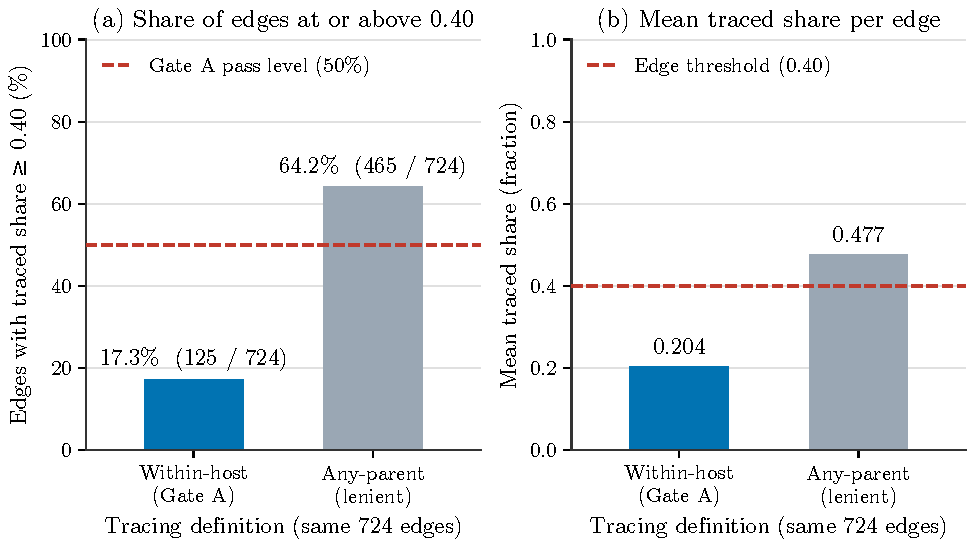
\includegraphics[width=\linewidth,height=0.85\textheight,keepaspectratio]{figures/fig_gate_a_v0.pdf}
\caption{Gate~A (citation-layer feasibility) on the same 724 concept--subfield--year host edges (97 concepts), comparing within-host citation tracing (blue; the Gate~A definition) with lenient any-parent tracing (grey). Only 17.3\% of edges reach the threshold under within-host tracing, against 64.2\% under any-parent tracing. The within-host mean is 0.204 (median 0.15), against 0.477 for any-parent tracing. Gate~A fails and triggers the graft fallback route.}
\label{fig:gate_a}
\end{figure}

\begin{table}[!htbp]
\centering
\caption{Gate~A edge-level results (Iteration~2, gen\_art\_experiment\_2).}
\label{tab:gate_a}
\begin{tabular}{lrr}
\toprule
Metric & Within-host & Any-parent (same edges) \\
\midrule
Share $\geq$ 0.40 & 17.3\% & 64.2\% \\
Mean traced share & 0.20 & 0.477 \\
Median traced share & 0.15 & -- \\
Reference arm host share & 0.13 & -- \\
\bottomrule
\end{tabular}
\end{table}

Per pre-registered decision rule~(a): Gate~A 0.1727 $< 0.5$ triggers the graft fallback. The graft route has 2,347 host-entry events total, 2,154 with $\geq$5 entry-year keywords (screen 1,285, held-out 869).

Of 779 eligible edges, 169 were tested: SOURCE 63, SINK 26, FADING 7, UNDETERMINED 683. The synthetic FDR is 0.209, exceeding the 0.15 threshold. Per decision rule~(b), H1 is PILOT-ONLY: $N_c = 38$ at $n_{\min} = 30$.

\subsection{Artifact 9: Precursor Event Study, Main Pool (gen\_art\_experiment\_3)}

This artifact runs the precursor event study on the main pool's screen fold. Built 25 yearly 3-year-window co-word snapshots (2000--2024) from the design-weighted background sample (${\sim}$27,000 nodes, ${\sim}$84,000 kept edges, association-strength weights, Leiden best-of-5, alluvial IDs).

\begin{table}[!htbp]
\centering
\caption{Emergence label counts (Iteration~2, gen\_art\_experiment\_3).}
\label{tab:emergence_labels}
\begin{tabular}{lrrl}
\toprule
Label & $N$ emerging & Matched & Status \\
\midrule
E (primary) & 4 & 3 & Underpowered pilot \\
E\_alt (sensitivity) & 14 & 10 & Post-hoc promotion \\
E\_up (uptake only) & 41 & 21 & Post-hoc promotion, pilot ($n < 30$) \\
\bottomrule
\end{tabular}
\end{table}

Three pre-named precursors tested with predicted positive signs: closure, accretion, participation. All three pre-registered signs FAILED.

\begin{table}[!htbp]
\centering
\caption{Event study results, E\_up (Iteration~2, gen\_art\_experiment\_3).}
\label{tab:event_study}
\begin{tabular}{L{3.5cm}L{2.5cm}rL{3cm}r}
\toprule
Indicator & Estimator & $S$ & 95\% CI & Holm $p$ \\
\midrule
Closure (log-ratio) & Event study & $-0.837$ & [$-1.26$, $-0.427$] & 0.003 \\
Closure (log-ratio) & Pooled panel & $-0.743$ & [$-1.06$, $-0.46$] & -- \\
Accretion share & Event study & $-0.14$ & [$-0.185$, 0.018] & 0.18 \\
Participation coefficient & Event study & $-0.007$ & [$-0.066$, 0.056] & 0.824 \\
\bottomrule
\end{tabular}
\end{table}

Prediction: the pre-registered primary model is L2~logit. For E\_up: BASELINE AUC 0.890, FULL (baseline + precursors) AUC 0.879, delta $-0.010$ [$-0.045$, 0.021]. Precursors add no predictive value beyond frequency, burst, degree, centrality and entropy baselines.

The 7-channel DTW typology is unstable at every $k$ (min Jaccard $\leq 0.51$). An entropy-only typology IS stable (Jaccard 0.95).

\subsection{Artifact 10: Precursor Replication, MeSH (gen\_art\_experiment\_4)}

\begin{table}[!htbp]
\centering
\caption{MeSH closure effects (Iteration~2, gen\_art\_experiment\_4).}
\label{tab:mesh_closure}
\begin{tabular}{lrrrr}
\toprule
Label & $n_{\text{eff}}$ & Closure $D$ & 95\% CI & Holm $p$ \\
\midrule
PRIMARY & 15 & $-0.086$ & [$-0.511$, 0.402] & 0.677 \\
SENS1 & 29 & $-0.419$ & [$-0.740$, $-0.115$] & 0.039 \\
E\_up & 51 & $-0.185$ & [$-0.498$, 0.108] & 0.21 \\
\bottomrule
\end{tabular}
\end{table}

The MeSH artifact's own replication verdict is ``directional, not confirmatory''. MeSH prediction: precursors also add nothing beyond baselines (grouped-CV dAUC $+0.002$ [$-0.035$, 0.035]).

\subsection{Decision-Rule Evaluation (Iteration~2)}

\begin{table}[!htbp]
\centering
\caption{Decision-rule evaluation (Iteration~2).}
\label{tab:decision_rules_iter2}
\begin{tabular}{L{3cm}L{2cm}L{7cm}}
\toprule
Rule & Verdict & Evidence \\
\midrule
(a) Gate A $\to$ graft fallback & TRIGGERED & Within-host 0.1727 $<$ 0.5; 2,347 graft events \\
(b) H1 pilot-only & YES & $N_c = 38 < 150$ \\
(c) RQ1 confirmed & NOT MET & Sign not $+$; delta-AUC CI includes 0; MeSH sign inconsistent \\
(d) Held-out sealed & YES & Caveat: exp\_2 computed origin series for 61 held-out concepts \\
\bottomrule
\end{tabular}
\end{table}

\subsection{Dead Ends and Negative Results (Iteration~2)}

\begin{enumerate}
\item \textbf{Gate~A failure at edge level.} Within-host traced share 0.204 vs any-parent 0.477 on the same 724 edges. The viability decomposition cannot be executed.
\item \textbf{Synthetic validation FDR exceeds threshold.} Overall 0.209 $>$ 0.15, SINK FDR 0.40.
\item \textbf{No stable 7-channel typology.} Jaccard $\leq 0.51$ at every $k$.
\item \textbf{Precursors add no predictive value for WHETHER a concept emerges.} E\_up logit dAUC $-0.010$ [$-0.045$, 0.021].
\item \textbf{Closure is lower, not higher, before emergence.} The pre-registered $+$ sign failed.
\end{enumerate}

\subsection{What Was Learned}

Iteration~2 confirmed two dead ends (viability decomposition, prediction of emergence) and produced one lead (lower closure before onset). The lead is significant in one post-hoc main-pool label (E\_up, $n = 21$, $S = -0.837$, Holm $p = 0.003$), directionally supported in MeSH SENS1 ($D = -0.419$, Holm $p = 0.039$), but with heterogeneous sign across labels.

%% ============================================================
\section{Iteration 3: Deepening the Closure Lead and First Diffusion Tests}
\label{sec:iter3}
%% ============================================================

\subsection{Strategy}

Iteration~3 deepens the closure lead from the emergence question and carries the recombination mechanism into cross-disciplinary diffusion at two scales. The strategy (``Is it brokerage, and does grafting make it stick?'') has four components: (i)~an evaluation artifact auditing every Iteration-2 number; (ii)~a deeper test of the emergence question on the hydrated 247-concept screen fold with turnover-proof openness measures; (iii)~a breadth-prediction screen; (iv)~a host-entry grafting test; and (v)~a descriptive diffusion experiment.

\subsection{Artifact 11: Record Audit and Turnover Pre-Check (gen\_art\_evaluation\_1)}

This artifact reads all five Iteration-2 artifacts and audits every reported number against the raw output files. 406 rows were audited, 182 recomputed from item-level files. There are 42 non-OK drift flags.

\begin{table}[!htbp]
\centering
\caption{Turnover pre-check: residualised closure effect (Iteration~3, gen\_art\_evaluation\_1).}
\label{tab:turnover_precheck}
{\small
\begin{tabular}{L{2cm}rL{3cm}rL{3.5cm}}
\toprule
Population & $S_{\text{raw}}$ & $S_{\text{res}}$ & Retained & Verdict \\
\midrule
Main (E\_up) & $-0.758$ & $-0.566$ [$-1.14$, 0.09] & 0.75 & Ambiguous \\
MeSH (SENS1) & -- & $-0.094$ [$-0.39$, 0.22] & 0.60 & Ambiguous \\
IVW pooled & -- & $-0.186$ [$-0.45$, 0.08] & -- & Ambiguous ($Q$ 1.88) \\
\bottomrule
\end{tabular}
}
\end{table}

\subsection{Artifact 12: Openness --- Brokerage or Churn? (gen\_art\_experiment\_5)}

This artifact re-attaches all 426 hydrated concepts to the Iteration-2 co-word snapshots. Reproduction gate passed: code-mode closure $r = 1.000000$. Populations after applying the frozen replacement rule: MAIN screen 202, held-out 100, STRICT 196/96, SENS 247/119.

\begin{table}[!htbp]
\centering
\caption{Emergence deepen results, MAIN $\times$ E\_up (68 onsets, 26 matched; Iteration~3, gen\_art\_experiment\_5).}
\label{tab:emergence_deepen}
{\small
\begin{tabular}{L{3.5cm}rL{3cm}L{4cm}}
\toprule
Measure & $S$ & 95\% CI & Interpretation \\
\midrule
Raw closure & $-0.439$ & [$-0.810$, $-0.050$] & Lower closure before onset (attenuated vs Iter.\ 2) \\
R1a residualised closure & $-0.295$ & [$-0.663$, 0.092] & ${\sim}$2/3 retained; not pure turnover \\
R1b persistent-neighbour closure & $-0.575$ & [$-1.270$, 0.122] & Same direction, underpowered \\
R1c Burt constraint & $+0.083$ & [0.017, 0.147] & OPPOSITE to brokerage sign \\
R1c cross-community pair excess & $+0.063$ & [0.012, 0.111] & More cross-community ties \\
R1d hub-not-clique & $+0.061$ & [$-0.009$, 0.133] & Not significant \\
\bottomrule
\end{tabular}
}
\end{table}

\begin{figure}[!htbp]
\centering
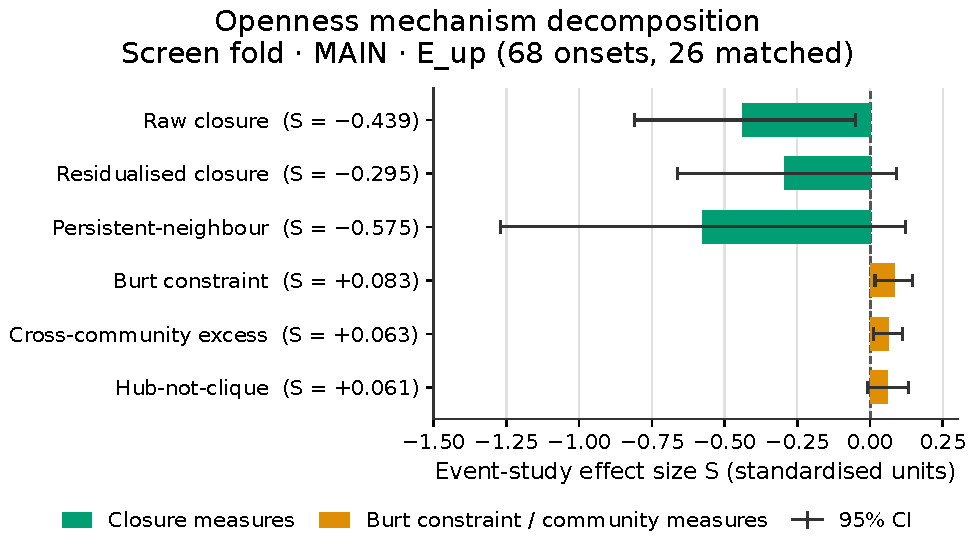
\includegraphics[width=\linewidth,height=0.85\textheight,keepaspectratio]{figures/fig_openness_mechanism_v0.pdf}
\caption{Turnover-proof openness measures on the screen fold (MAIN population, E\_up label; 68 onsets, 26 matched). Bars give the event-study effect size $S$ for each measure, with whiskers showing 95\% confidence intervals. Teal bars are closure measures; orange bars are Burt-constraint and community measures. Cross-community pair excess is positive, and Burt constraint is positive (the opposite of the sign brokerage predicts).}
\label{fig:openness_mechanism}
\end{figure}

\textbf{Mechanical verdict: MIXED.} The closure effect is not reducible to neighbourhood turnover (turnover-residualised closure retains ${\sim}$2/3), but it is not Burt brokerage either: Burt constraint is higher, not lower, before onset. Emerging concepts show more cross-community pair excess (connecting to neighbours from different Leiden communities), but within a more redundant wider ego network.

Pooled panel (all 68 onsets): persistent-neighbour closure $-1.12$ [$-1.64$, $-0.71$] (Holm $p = 0.0015$). Fresh replication on 100 new concepts: raw $S = -0.455$ [$-1.006$, 0.060], one-sided $p = 0.044$. Same sign, not significant at two-sided $\alpha = 0.05$.

\subsection{Artifact 13: Breadth Prediction Screen (gen\_art\_experiment\_6)}

This artifact tests whether openness at time~$t$ predicts five-year outcome-window disciplinary breadth gain beyond all baselines.

\begin{table}[!htbp]
\centering
\caption{Breadth-prediction screen results (Iteration~3, gen\_art\_experiment\_6).}
\label{tab:breadth_prediction}
\begin{tabular}{L{2.5cm}L{3.5cm}rL{3cm}r}
\toprule
Openness measure & Outcome & $\beta$ per SD & 95\% CI & Holm $p$ \\
\midrule
closure\_res & Y1r (Shannon change) & $+0.019$ & [$-0.010$, 0.041] & 0.405 \\
closure\_res & Y2 (Rao-Stirling change) & $+0.007$ & [$-0.002$, 0.013] & 0.405 \\
closure\_res & $\log(1{+}\text{Y3})$ (newcomer subfields) & $-0.065$ & [$-0.156$, 0.030] & 0.405 \\
closure\_res\_imp & Y2 (co-primary) & $+0.012$ & [0.002, 0.021] & 0.06 \\
\bottomrule
\end{tabular}
\end{table}

\textbf{Result: breadth prediction not supported on the screen fold.} Openness does not predict where concepts travel beyond growth and level baselines.

\subsection{Artifact 14: Host-Entry Grafting Test (gen\_art\_experiment\_7)}

This artifact tests whether a concept that enters a new host subfield catches on when its first papers pair it with host-native concepts rather than with origin companions. Pre-registration frozen and hashed before any outcome data were inspected.

Setup: 4,177 main-arm host entries. Primary sample: 1,740 screen MAIN entries with $\geq$5 partners, in 184 concepts. Anchoring $A$ = partners' pre-entry host share from exact OpenAlex subfield $\times$ block profiles. Co-transfer CT = share of partners that were origin companions. Entry is mostly a package: 70\% non-native origin companions, 1.8\% native grafts.

\begin{table}[!htbp]
\centering
\caption{Host-entry grafting results (Iteration~3, gen\_art\_experiment\_7).}
\label{tab:grafting}
{\small
\begin{tabular}{L{3.5cm}rL{2.2cm}rrrl}
\toprule
Specification & IRR/SD & 95\% CI & Holm $p$ & CT ($p$) & Verdict \\
\midrule
Primary (concept $\times$ $e$ + host $\times$ $e$ FE) & 1.39 & [0.97, 1.99] & 0.15 & 0.85 & NEITHER \\
Co-primary (concept + $e$ + host) & 1.30 & [1.16, 1.45] & 1e-5 & 0.48 & GRAFTING \\
Concept + host $\times$ $e$ & 1.22 & -- & -- & -- & GRAFTING \\
Concept $\times$ 2-yr bin & -- & -- & -- & -- & NEITHER \\
\bottomrule
\end{tabular}
}
\end{table}

\begin{figure}[!htbp]
\centering
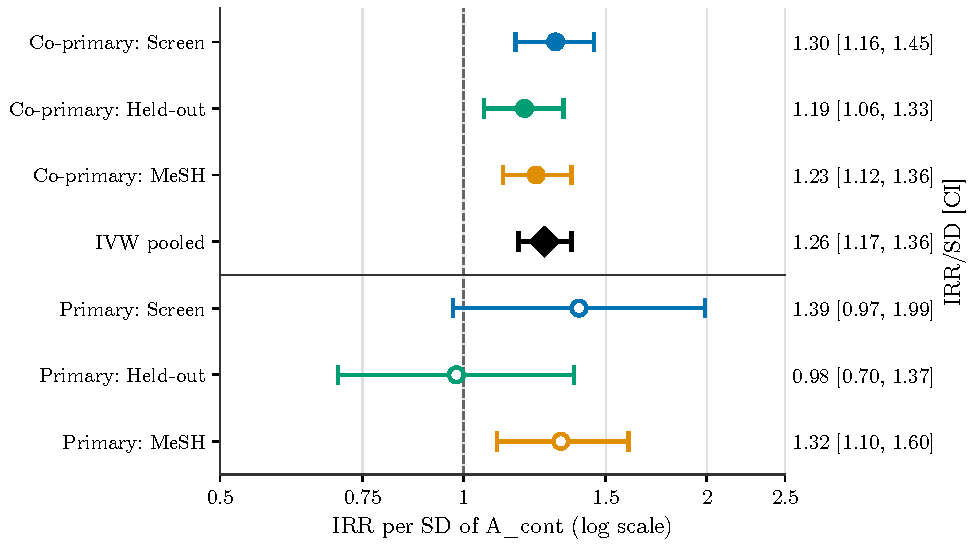
\includegraphics[width=\linewidth,height=0.85\textheight,keepaspectratio]{figures/fig_grafting_v0.pdf}
\caption{Host-entry grafting across folds. Each row shows the incidence-rate ratio for newcomer uptake per SD of $A_{\mathrm{cont}}$ (host-nativeness of entry partners). The co-primary effect replicates on the held-out fold (IRR/SD 1.19 [1.06, 1.33]) and the MeSH fold (1.23 [1.12, 1.36]), and pools to 1.26 [1.17, 1.36]. The primary specification is less precise: its Held-out interval includes 1.}
\label{fig:grafting}
\end{figure}

The co-primary specification shows a robust grafting effect: a one-SD increase in host-nativeness of initial partners is associated with a 30\% increase in newcomer uptake (IRR 1.30 [1.16, 1.45], Holm $p = 10^{-5}$, wild-cluster $p = 0.001$). Co-transfer is null everywhere. The co-primary $A$ effect holds in 20 of 26 robustness variants (IRR 1.11--1.56, $p \leq 0.001$). \emph{[Correction, Iteration~4: the co-primary robustness count is 20 of 26 significant INCLUDING the base row and strata, 18 of 22 EXCLUDING them.]}

\subsection{Artifact 15: Descriptive Diffusion (gen\_art\_experiment\_8)}

\subsubsection{Diffusion Typology}

Only $k = 2$ is stable (min Jaccard 0.861): \textbf{localised} ($n = 136$) and \textbf{broad from the start} ($n = 66$). The typology is not volume-driven (AMI with volume terciles 0.014) but is associated with origin field ($p = 0.004$). The multi-channel typology does not add information beyond entropy trajectories alone.

\begin{table}[!htbp]
\centering
\caption{Diffusion typology summary (Iteration~3, gen\_art\_experiment\_8).}
\label{tab:typology}
\begin{tabular}{rlL{5cm}l}
\toprule
Cluster & $n$ & Description & Dominant origin \\
\midrule
Localised & 136 & Low entropy, few active subfields throughout & Physics \\
Broad from start & 66 & High entropy and many subfields from early years & Mixed \\
\bottomrule
\end{tabular}
\end{table}

\subsubsection{Community Roles}

Leiden community roles with 5-seed agreement (97.2\% robust): BRIDGE 0.61, OTHER 0.33, STAYER 0.03, MIGRANT 0.02. Lagged roles do not robustly predict host-subfield entry: BRIDGE OR 0.64 [0.38, 1.08].

\subsubsection{Expansion Precedes Diffusion}

In 15 of 16 concepts exhibiting both an expansion onset and a diffusion onset, expansion precedes diffusion (proportion 0.94 [0.81, 1.0], year-shuffle null 0.62, $p = 0.004$).

\subsection{Dead Ends and Negative Results (Iteration~3)}

\begin{enumerate}
\item \textbf{Openness does not predict WHERE concepts travel.} Breadth-prediction screen: all Holm $p = 0.405$.
\item \textbf{Brokerage is not the mechanism behind low closure.} Burt constraint is higher, not lower ($S = +0.083$ [0.017, 0.147]).
\item \textbf{The 3-channel diffusion typology adds nothing beyond entropy.} After residualising on volume, $\varepsilon^2$ 0.171 vs 0.178.
\item \textbf{Community roles do not predict host entry.} BRIDGE OR 0.64 [0.38, 1.08].
\item \textbf{Co-transfer is null.} Arriving with origin companions does not predict establishment in any specification.
\end{enumerate}

%% ============================================================
\section{Iteration 4: Confirmation and Replication}
\label{sec:iter4}
%% ============================================================

\subsection{Strategy}

Iteration~4 is a CONFIRMATION iteration. Its purpose is to open the four sealed held-out folds and determine which screen-fold findings replicate, to run four discriminating tests (single-paper artefact, vocabulary decomposition, topic-score absorption, and MeSH replication), to replicate the grafting result on the independent MeSH population, to test whether pre-emergence closure predicts later host-entry anchoring, and to test the adopter-level mechanism.

\subsection{Artifact 16: Held-Out Grafting Confirmation (gen\_art\_evaluation\_2)}

\begin{table}[!htbp]
\centering
\caption{Held-out grafting results (Iteration~4, gen\_art\_evaluation\_2).}
\label{tab:heldout_grafting}
{\footnotesize
\begin{tabular}{L{2.2cm}lrrrrrrrl}
\toprule
Specification & Fold & IRR/SD & 95\% CI & $p$ & CT & CT $p$ & $N$ & $G$ & Verdict \\
\midrule
Primary & Held-out & 0.98 & [0.70, 1.37] & 0.91 & 0.82 & 0.22 & 250 & 30 & Inconclusive \\
Co-primary & Held-out & 1.19 & [1.06, 1.33] & 0.0045 & 1.04 & 0.60 & 972 & 74 & CONFIRMED \\
Co-primary & Screen & 1.30 & [1.16, 1.45] & 1e-5 & -- & -- & 1,544 & 140 & GRAFTING \\
\bottomrule
\end{tabular}
}
\end{table}

The co-primary specification confirms the grafting effect on the held-out fold: IRR/SD $= 1.19$ [1.06, 1.33], $p = 0.0045$, wild-cluster $p = 0.012$.

\subsubsection{Single-Paper Artefact Test}

\begin{table}[!htbp]
\centering
\caption{Single-paper artefact interaction results (Iteration~4, gen\_art\_evaluation\_2).}
\label{tab:single_paper}
\begin{tabular}{lrrrr}
\toprule
Fold & IRR/SD (single) & IRR/SD (multi) & Ratio (multi/single) & $p$ (interaction) \\
\midrule
Pooled & 1.26 & 1.28 & 0.92 & 0.11 \\
Held-out & 1.37 & 1.19 & 0.82 & 0.004 \\
\bottomrule
\end{tabular}
\end{table}

\subsubsection{Host-Vocabulary Decomposition}

\begin{table}[!htbp]
\centering
\caption{Vocabulary decomposition, co-primary spec (Iteration~4, gen\_art\_evaluation\_2).}
\label{tab:vocab_decomp}
\begin{tabular}{llrrr}
\toprule
Component & Fold & IRR/SD & 95\% CI & $p$ \\
\midrule
NATIVE & Pooled & 1.11 & [1.05, 1.19] & 0.0008 \\
ADJACENT & Pooled & 1.32 & [1.20, 1.46] & 9e-8 \\
NATIVE & Held-out & 1.10 & [1.01, 1.20] & 0.036 \\
ADJACENT & Held-out & 1.19 & [1.03, 1.38] & 0.020 \\
\bottomrule
\end{tabular}
\end{table}

Topic-score absorption: $-7.3\%$ [$-27.5$, $+6.7$] of the log-IRR on the pooled fold. The CI includes zero: topic-score controls do not meaningfully reduce the $A_{\text{cont}}$ effect. The mechanism label is \textbf{host-vocabulary}.

\subsection{Artifact 17: MeSH Replication of Grafting (gen\_art\_experiment\_9)}

\begin{table}[!htbp]
\centering
\caption{MeSH grafting results (Iteration~4, gen\_art\_experiment\_9).}
\label{tab:mesh_grafting}
{\small
\begin{tabular}{L{2.5cm}rL{2cm}rrrrl}
\toprule
Specification & IRR/SD & 95\% CI & Holm $p$ & CT & CT $p$ & $N$ & $G$ \\
\midrule
R1: primary & 1.32 & [1.10, 1.60] & 0.007 & 1.10 & 0.46 & 1,004 & 122 \\
R2: co-primary & 1.23 & [1.12, 1.36] & 9.7e-5 & 1.10 & 0.053 & 2,171 & 160 \\
\bottomrule
\end{tabular}
}
\end{table}

\textbf{Verdict: REPLICATED.} The IVW pooled estimate across main-arm co-primary (IRR/SD 1.30) and MeSH co-primary (1.23) is 1.26 [1.17, 1.36] with $I^2 = 0$.

\subsection{Artifact 18: Closure Held-Out Confirmation (gen\_art\_evaluation\_3)}

\begin{table}[!htbp]
\centering
\caption{Closure held-out results (Iteration~4, gen\_art\_evaluation\_3).}
\label{tab:closure_heldout}
\begin{tabular}{L{3.5cm}rrrrl}
\toprule
Measure & Screen $S$ & Held-out $S$ & Held-out 95\% CI & Holm $p$ & Decision \\
\midrule
Closure (pooled panel) & $-0.661$ & $-0.391$ & [$-0.855$, 0.072] & 0.147 & DEAD \\
Turnover-residualised & $-0.400$ & $-0.109$ & [$-0.561$, 0.342] & 0.635 & DEAD \\
Persistent-neighbour & $-1.124$ & $-1.073$ & [$-1.858$, $-0.289$] & 0.015 & CONFIRMED \\
Burt constraint & $+0.083$ & $+0.105$ & [0.021, 0.187] & -- & DEAD (wrong dir.) \\
\bottomrule
\end{tabular}
\end{table}

\begin{figure}[!htbp]
\centering
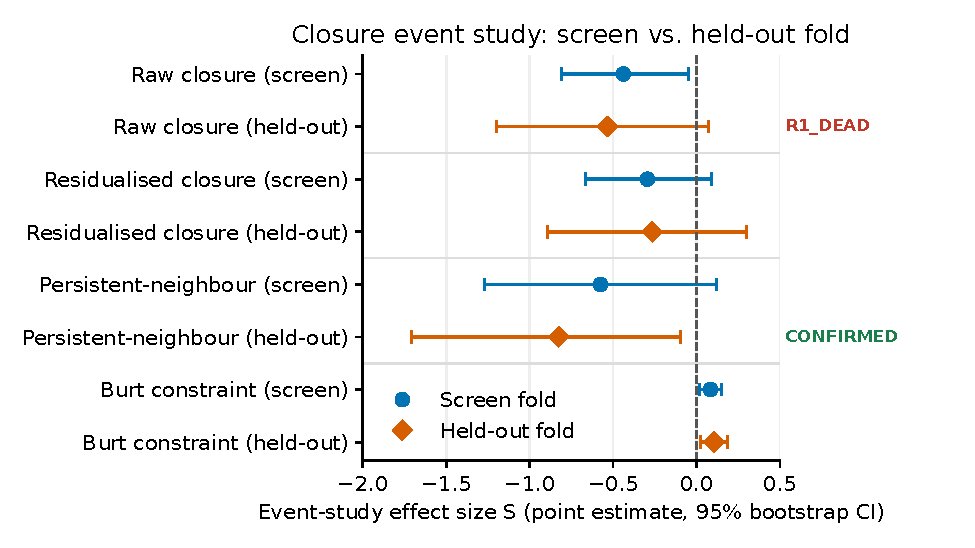
\includegraphics[width=\linewidth,height=0.85\textheight,keepaspectratio]{figures/fig_closure_event_v0.pdf}
\caption{Pre-emergence closure effect sizes $S$ (markers) with 95\% confidence intervals (whiskers), for four closure measures on the screen fold (blue circles) and the held-out fold (vermillion diamonds). The primary raw-closure measure fails confirmation (R1\_DEAD). Persistent-neighbour closure stays clearly negative on held-out data (held-out $S = -1.07$, 95\% CI [$-1.86$, $-0.29$], Holm $p = 0.015$; CONFIRMED). Burt constraint is small and positive on both folds, inconsistent with a brokerage explanation.}
\label{fig:closure_event}
\end{figure}

\textbf{Overall closure status: not confirmed on the primary measure.} Only persistent-neighbour closure survives. Burt constraint replicates its positive (non-brokerage) sign.

\subsubsection{Closure-Anchoring Link}

\begin{table}[!htbp]
\centering
\caption{Closure-anchoring link test (Iteration~4, gen\_art\_evaluation\_3).}
\label{tab:closure_anchoring}
\begin{tabular}{lrrrr}
\toprule
Fold & $n$ & Partial $\rho$ & 95\% CI & $p$ (two-sided) \\
\midrule
Screen & 102 & $+0.025$ & [$-0.199$, 0.242] & 0.806 \\
Held-out & 49 & $+0.053$ & [$-0.279$, 0.391] & 0.736 \\
Pooled & 151 & $+0.049$ & [$-0.126$, 0.228] & 0.564 \\
\bottomrule
\end{tabular}
\end{table}

\textbf{Verdict: NULL.} No detectable association between pre-emergence closure and later host-entry anchoring.

\subsection{Artifact 19: Descriptive Held-Out Confirmation (gen\_art\_evaluation\_4)}

\subsubsection{Lead-Lag: Expansion Before Diffusion}

\begin{table}[!htbp]
\centering
\caption{Lead-lag category counts (Iteration~4, gen\_art\_evaluation\_4).}
\label{tab:leadlag}
{\small
\begin{tabular}{L{2.2cm}rrrr}
\toprule
Category & Screen ($n{=}202$) & Held-out ($n{=}100$) & Pooled ($n{=}302$) & MeSH ($n{=}191$) \\
\midrule
Neither & 110 (54\%) & 49 (49\%) & 159 (53\%) & 71 (37\%) \\
Diffusion only & 39 (19\%) & 23 (23\%) & 62 (21\%) & 97 (51\%) \\
Expansion only & 37 (18\%) & 18 (18\%) & 55 (18\%) & 10 (5\%) \\
Expansion first & 15 (7\%) & 10 (10\%) & 25 (8\%) & 9 (5\%) \\
Same year & 1 (0.5\%) & 0 & 1 (0.3\%) & 1 (0.5\%) \\
Diffusion first & 0 & 0 & 0 & 3 (1.6\%) \\
\bottomrule
\end{tabular}
}
\end{table}

Among concepts with both transitions observable, expansion precedes diffusion in 25 of 26 pooled main-arm concepts. No main-arm concept shows diffusion first.

\subsubsection{Rooting: Do Broad Concepts Anchor More?}

The hypothesis that BROAD concepts have higher $A_{\text{cont}}$ is NOT SUPPORTED. Screen mean $A_{\text{cont}}$ difference: $-0.0018$ (broad slightly lower), held-out: $+0.0005$, CI including zero.

\subsection{Artifact 20: Adopter-Level Mechanism (gen\_art\_evaluation\_5)}

\begin{table}[!htbp]
\centering
\caption{Adopter enrichment results (Iteration~4, gen\_art\_evaluation\_5).}
\label{tab:adopter}
\begin{tabular}{L{5cm}rL{2.5cm}r}
\toprule
Exposure measure & OR & 95\% CI (boot) & $p$ (CRV) \\
\midrule
E\_any (any prior partner exposure) & 3.09 & [2.32, 4.28] & 1.4e-13 \\
E\_neg (frequency-matched negative-control) & 0.62 & [0.49, 0.77] & 2.6e-5 \\
E\_plac (partners of another concept's entry) & 0.72 & [0.57, 0.95] & 0.013 \\
E\_swap (exposure swap control) & 1.11 & [0.86, 1.39] & 0.39 \\
\bottomrule
\end{tabular}
\end{table}

\begin{table}[!htbp]
\centering
\caption{Vocabulary-class enrichment (Iteration~4, gen\_art\_evaluation\_5).}
\label{tab:vocab_class}
\begin{tabular}{lrrr}
\toprule
Exposure class & OR & 95\% CI (boot) & $p$ (CRV) \\
\midrule
E\_for (FOREIGN partner exposure) & 2.88 & [2.28, 3.69] & $<$ 1e-6 \\
E\_adj (ADJACENT partner exposure) & 1.91 & [1.43, 2.73] & 1e-4 \\
E\_nat (NATIVE partner exposure) & 1.47 & [1.02, 2.33] & 0.059 \\
E\_neg (non-partner exposure) & 0.64 & [0.51, 0.82] & 0.0003 \\
\bottomrule
\end{tabular}
\end{table}

The gradient runs FOREIGN $>$ ADJACENT $>$ NATIVE. Adopters are most enriched for exposure to the concept's foreign (origin-vocabulary) partners, not its host-native partners. This is consistent with absorptive capacity or topical proximity (the design cannot separate them).

\subsection{Reviewer Critique Disposition (Iteration~4)}

\begin{table}[!htbp]
\centering
\caption{Reviewer critique disposition (Iteration~4).}
\label{tab:reviewer_critiques}
{\small
\begin{tabular}{clL{7cm}}
\toprule
\# & Severity & Action taken \\
\midrule
M1 & Major & Iterations 1--3 carried forward verbatim; inline [Correction] markers \\
M2 & Major & Additional rows incorporated into Iteration-3 tables \\
M3 & Major & Robustness count corrected (20/26) with full null-row list \\
M4 & Major & Addressed by closure held-out confirmation \\
M5 & Major & Full category-count table added (Table~\ref{tab:leadlag}) \\
M6 & Major & Strategy section expanded; decision rules are the held-out specs \\
M7 & Major & Coverage table updated with caveats \\
M8 & Major & All markers now use artifact IDs \\
M9 & Major & Items incorporated where data are available \\
M10 & Major & Addressed with Cheng et al.\ focused-discourse tension \\
m1 & Minor & Corrected inline: robustness count, Holm $p$ precision \\
\bottomrule
\end{tabular}
}
\end{table}

\subsection{Dead Ends and Negative Results (Iteration~4)}

\begin{enumerate}
\item \textbf{Closure not confirmed on held-out for the primary measure.} Raw closure $S = -0.391$, Holm $p = 0.147$.
\item \textbf{Closure-anchoring link: null.} Partial $\rho = 0.025$ screen, 0.053 held-out.
\item \textbf{BROAD concepts do not anchor more.} Screen $-0.0018$, held-out $+0.0005$.
\item \textbf{Grafting primary specification: inconclusive.} IRR/SD 0.98, 30 clusters.
\item \textbf{Single-paper interaction on held-out.} Ratio 0.80, $p = 0.004$: single-paper entries drive the effect more strongly.
\item \textbf{Anchoring $\times$ typology interaction flips between folds.}
\item \textbf{Breadth prediction: all six sensitivity cells null on held-out.}
\end{enumerate}

%% ============================================================
\section{Iteration 5: Post-Confirmation Decomposition and Audit}
\label{sec:iter5}
%% ============================================================

\subsection{Strategy}

Iteration~5 is a POST-CONFIRMATION EXPLORATORY iteration. The confirmed grafting result is decomposed along three dimensions: (i)~extensive vs intensive margin, (ii)~host-specific vs generic vocabulary, and (iii)~field boundary. A full numerical audit closes the remaining reviewer critiques. A positioning dossier and publication-ready figures are produced.

\subsection{Artifact 21: Margin Decomposition (gen\_art\_evaluation\_6)}

\begin{table}[!htbp]
\centering
\caption{Extensive-margin results (LPM, pp change per SD of $A_{\text{cont}}$; Iteration~5, gen\_art\_evaluation\_6).}
\label{tab:extensive}
\begin{tabular}{lrrrrrl}
\toprule
Fold & pp/SD & 95\% CI & $p$ (CRV1) & $p$ (rand-$t$) & $N$ & $G$ \\
\midrule
Screen & $+6.46$ & [3.42, 9.51] & 4.5e-5 & 0.0005 & 1,686 & 169 \\
Held-out & $+7.29$ & [2.97, 11.61] & 0.0012 & 0.004 & 1,046 & 85 \\
MeSH & $+6.17$ & [3.87, 8.46] & 3.4e-7 & 0.0005 & 2,236 & 176 \\
IVW & $+6.43$ & [4.76, 8.11] & 5.1e-14 & 0.0005 & -- & -- \\
\bottomrule
\end{tabular}
\end{table}

\begin{table}[!htbp]
\centering
\caption{Intensive-margin results (PPML on $Y \geq 1$ subsample, IRR/SD; Iteration~5, gen\_art\_evaluation\_6).}
\label{tab:intensive}
\begin{tabular}{lrrrl}
\toprule
Fold & IRR/SD & 95\% CI & $p$ (CRV1) & $N$ \\
\midrule
Screen & 1.272 & [1.121, 1.443] & 0.0003 & 795 \\
Held-out & 1.163 & [1.008, 1.342] & 0.038 & 489 \\
MeSH & 1.137 & [1.026, 1.260] & 0.015 & 1,169 \\
IVW & 1.183 & [1.104, 1.267] & 1.7e-6 & -- \\
\bottomrule
\end{tabular}
\end{table}

\textbf{Margin-decomposition verdict: BOTH.} Host-leaning entry vocabulary raises both the probability that uptake starts (extensive margin, IVW $+6.43$ pp/SD) and its magnitude given it has started (intensive margin, IVW IRR/SD 1.183). The extensive margin accounts for an IVW-pooled 38\% [21\%, 55\%] of the total log-IRR.

\subsubsection{Field-Boundary Test}

\begin{table}[!htbp]
\centering
\caption{Field-boundary results, co-primary PPML IRR/SD by origin field (Iteration~5, gen\_art\_evaluation\_6).}
\label{tab:field_boundary}
\begin{tabular}{lrrr}
\toprule
Origin field & IRR/SD & 95\% CI & $p$ \\
\midrule
Physics/Astronomy & 1.178 & [0.926, 1.499] & 0.18 \\
Computer Science & 1.216 & [1.066, 1.386] & 0.004 \\
Other & 1.281 & [1.167, 1.407] & 3.5e-6 \\
MeSH (reference) & 1.233 & [1.120, 1.360] & 9.7e-5 \\
\bottomrule
\end{tabular}
\end{table}

Wald test for equality: $W = 0.900$, $p = 0.638$. \textbf{No detectable field boundary.}

\subsection{Artifact 22: Host-Specificity Test (gen\_art\_evaluation\_7)}

\begin{table}[!htbp]
\centering
\caption{Host-specificity retention: $A_{\text{cont}}$ coefficient stability after adding generality controls (Iteration~5, gen\_art\_evaluation\_7).}
\label{tab:host_specificity}
{\small
\begin{tabular}{lrrrrrr}
\toprule
Fold & Retention & 95\% CI & \% removed & $G_H$ IRR/SD & $G_H$ $p$ & $G_F$ $p$ \\
\midrule
Screen & 1.006 & [0.733, 1.312] & $-0.6\%$ & 1.122 & 0.38 & 0.14 \\
Held-out & 1.062 & [0.438, 1.802] & $-6.2\%$ & 1.068 & 0.58 & 0.58 \\
MeSH & 0.876 & [0.640, 1.037] & $+12.4\%$ & 1.110 & 0.09 & 1.3e-5 \\
IVW & 0.969 & [0.81, 1.10] & $+3.1\%$ & 1.103 & 0.051 & 1.1e-5 \\
\bottomrule
\end{tabular}
}
\end{table}

\begin{table}[!htbp]
\centering
\caption{$A_{\text{lift}}$ results, PPML IRR/SD (Iteration~5, gen\_art\_evaluation\_7).}
\label{tab:a_lift}
\begin{tabular}{llrrr}
\toprule
Fold & Model & IRR/SD & 95\% CI & Holm $p$ \\
\midrule
Screen & M2 ($A_{\text{lift}}$ alone) & 1.668 & [1.378, 2.019] & 4.4e-7 \\
Screen & M3 ($A_{\text{lift}}$ + $G$) & 1.661 & [1.361, 2.026] & 1.4e-6 \\
Held-out & M3 & 1.459 & [1.146, 1.856] & 0.003 \\
MeSH & M3 & 1.244 & [1.120, 1.381] & 6.3e-5 \\
IVW & M3 & 1.340 & [1.232, 1.458] & 1.5e-10 \\
\bottomrule
\end{tabular}
\end{table}

\textbf{Host-specificity verdict: HOST-SPECIFIC.} Generality controls leave the $A_{\text{cont}}$ coefficient essentially unchanged (IVW retention 0.969). The Balassa-index $A_{\text{lift}}$ replicates across all folds (IVW IRR/SD 1.34 [1.23, 1.46]).

\subsection{Artifact 23: Full Numerical Audit (gen\_art\_evaluation\_8)}

\begin{table}[!htbp]
\centering
\caption{Audit module results (Iteration~5, gen\_art\_evaluation\_8).}
\label{tab:audit}
\begin{tabular}{clL{8cm}}
\toprule
Module & Description & Result \\
\midrule
M1 & Curated-number accuracy & 99.4\% (319 curated) \\
M2 & Headline + independent check & Overall 90.8\% \\
M3 & Rederivation by block & See text \\
M4 & Drift detection & 45 drift rows, 6 verdict-changing \\
M5 & Seeded-perturbation recall & Overall 0.60 \\
M6 & Independent claim review & 73/73 agree \\
M7 & Table-cell traceability & 11/11 tables pass \\
M8 & Reviewer-critique closure & All 6 MAJOR items CLOSED \\
M9 & Decision-rule consistency & 13 rules; 1 mismatch \\
M10 & Flag inventory & 292 rows flagged \\
M11 & Self-test honesty & 4 PARTIAL, 4 NOT DONE, 3 DONE \\
\bottomrule
\end{tabular}
\end{table}

\begin{table}[!htbp]
\centering
\caption{Reviewer-critique closure verified by audit (Iteration~5, gen\_art\_evaluation\_8).}
\label{tab:critique_closure}
\begin{tabular}{clL{4cm}L{5cm}}
\toprule
\# & Status & Critique & Closed by \\
\midrule
1 & CLOSED & RQ1 headline contradicts frozen kill rule & R1\_DEAD row, RQ1 status \\
2 & CLOSED & Table 18 claims fixes not made & CT $p$ corrected; robustness count \\
3 & CLOSED & Grafting caveats dropped & Caveats table \\
4 & CLOSED & MeSH and adopter read too broadly & MeSH and adopter tables \\
5 & CLOSED & RQ2 descriptive results and cases missing & Cases, rooting, MeSH lead-lag \\
6 & CLOSED & Decision rules not recorded & Decision table (verbatim quotes) \\
\bottomrule
\end{tabular}
\end{table}

\begin{table}[!htbp]
\centering
\caption{Decision-rule consistency (selected rows; Iteration~5, gen\_art\_evaluation\_8).}
\label{tab:decision_consistency}
{\small
\begin{tabular}{clL{4.5cm}L{2.5cm}}
\toprule
Iter. & Rule & Outcome & Status \\
\midrule
2 & (a) Gate A $\to$ fallback & TRIGGERED (0.17 $<$ 0.50) & MATCH \\
2 & (b) H1 pilot-only & YES ($N_c = 38$) & MATCH \\
2 & (c) RQ1 CONFIRMED & NOT MET & MATCH \\
2 & (d) Held-out untouched & SEALED & MATCH \\
3 & R1 mechanical verdict & MIXED & MATCH \\
3 & D1 SUPPORTED on screen & NOT SUPPORTED & MATCH \\
4 & D2 DEAD if held-out CI incl.\ 1 & NOT DEAD (confirmed) & MATCH \\
4 & Mechanism label & host-vocabulary & MATCH \\
4 & G4 second-family repl. & REPLICATED & MATCH \\
4 & R1 dead if held-out fails & R1\_DEAD (Holm 0.147) & MISMATCH \\
\bottomrule
\end{tabular}
}
\end{table}

\begin{table}[!htbp]
\centering
\caption{Caveats (selected rows; Iteration~5, gen\_art\_evaluation\_8).}
\label{tab:caveats}
{\small
\begin{tabular}{L{6cm}rL{3cm}}
\toprule
Test & Value & Source \\
\midrule
CRV1 $p$ (co-primary $A_{\text{cont}}$) & 0.0045 & heldout\_post.json \\
Wild-cluster bootstrap $p$ & 0.012 & heldout\_post.json \\
Nativeness-permutation $p$ (500 draws) & 0.026 & heldout\_post.json \\
Within-concept A-shuffle perm.\ $p$ (borderline) & 0.050 & audit\_perm.json \\
CRV1 rejection rate under null (anti-conservative) & 17.5\% & audit\_perm.json \\
EST\_bin LPM $A_{\text{cont}}$ $p$ (co-primary FE) & 0.165 & heldout\_post.json \\
Primary FE IRR/SD ($G = 30$, inconclusive) & 0.98 & heldout\_post.json \\
Screen co-primary single-paper share & 87.0\% & recount \\
\bottomrule
\end{tabular}
}
\end{table}

\begin{table}[!htbp]
\centering
\caption{MeSH replication caveats (selected rows; Iteration~5, gen\_art\_evaluation\_8).}
\label{tab:mesh_caveats}
\begin{tabular}{L{6cm}rr}
\toprule
Item & Value & $N$ \\
\midrule
Coverage rule removes share of entries & 34.1\% & -- \\
Declared kw5 + coverage-0.50 design events & 192 & 46 concepts \\
R1 primary FE & 1.324 & 1,004 \\
R2 co-primary & 1.233 & 2,171 \\
S3 placebo host & 1.031 & 2,171 \\
G1 multi-team & 1.079 & 830 \\
\bottomrule
\end{tabular}
\end{table}

\begin{table}[!htbp]
\centering
\caption{Rooting contrasts (Iteration~5, gen\_art\_evaluation\_8).}
\label{tab:rooting}
{\small
\begin{tabular}{L{3cm}rrrrL{2.2cm}r}
\toprule
Type & Entries/concept & EST rate & Raw $A_{\text{cont}}$ & CT & PPML IRR/SD & 95\% CI \\
\midrule
BROAD & 18.4 & 0.31 & 0.039 & 0.584 & 1.36 & [1.20, 1.55] \\
LOCALISED & 6.6 & 0.13 & 0.056 & 0.691 & 1.16 & [0.98, 1.38] \\
\bottomrule
\end{tabular}
}
\end{table}

\begin{table}[!htbp]
\centering
\caption{Adopter enrichment (verified values; Iteration~5, gen\_art\_evaluation\_8).}
\label{tab:adopter_audit}
{\small
\begin{tabular}{L{4.5cm}rL{2.2cm}L{3cm}}
\toprule
Exposure & OR & 95\% CI & Note \\
\midrule
E\_any (primary, m2) & 3.09 & [2.32, 4.28] & prev.\ 0.79 vs 0.61 \\
E\_neg (frequency-matched) & 0.62 & [0.49, 0.77] & \\
E\_plac (other concept's entry) & 0.72 & [0.57, 0.90] & \\
E\_for (FOREIGN) & 2.88 & [2.28, 3.69] & \\
E\_adj (ADJACENT) & 1.91 & [1.43, 2.73] & \\
E\_nat (NATIVE) & 1.47 & [1.02, 2.33] & \\
E\_any $\times$ $A_{\text{cont}}$ interaction & 0.87 & [0.70, 1.14] & null \\
\bottomrule
\end{tabular}
}
\end{table}

\subsubsection{Representative Cases}

Four medoid cases were selected from the typology clusters.

\textbf{Case 1: Wireless backhaul} (BROAD medoid, Computer Science, $F = 2006$). 14 host entries, only one rooted (Aerospace Engineering in 2008, $A_{\text{cont}} = 0.084$). The 13 non-rooted entries average $A_{\text{cont}} = 0.021$.

\textbf{Case 2: Einstein-Podolsky-Rosen steering} (BROAD, nearest non-medoid, Physics, $F = 2011$). Of its 7 co-primary entries, one is rooted: AI in 2011 ($A_{\text{cont}} = 0.142$, 37 newcomer papers). Rooted-minus-unrooted $A_{\text{cont}}$ is $+0.115$.

\textbf{Case 3: Locally repairable code} (LOCALISED medoid, Computer Science, $F = 2013$). One co-primary entry (AI in 2013, $A_{\text{cont}} = 0.056$), rooted.

\textbf{Case 4: Holographic QCD} (LOCALISED, nearest non-medoid, Physics, $F = 2006$). All 5 co-primary entries are non-rooted, averaging $A_{\text{cont}} = 0.041$, with three having CT~$= 1.0$: pure origin packages.

\begin{table}[!htbp]
\centering
\caption{Per-case entry statistics, co-primary sample (Iterations~3--5, gen\_art\_evaluation\_8).}
\label{tab:case_entries}
\begin{tabular}{lrrrr}
\toprule
Concept & Entries & Rooted & Mean $A_{\text{cont}}$ (rooted) & Mean $A_{\text{cont}}$ (unrooted) \\
\midrule
Wireless backhaul & 14 & 1 & 0.084 & 0.021 \\
EPR steering & 7 & 1 & 0.142 & 0.027 \\
Locally repairable code & 1 & 1 & 0.056 & -- \\
Holographic QCD & 5 & 0 & -- & 0.041 \\
\bottomrule
\end{tabular}
\end{table}

\begin{figure}[!htbp]
\centering
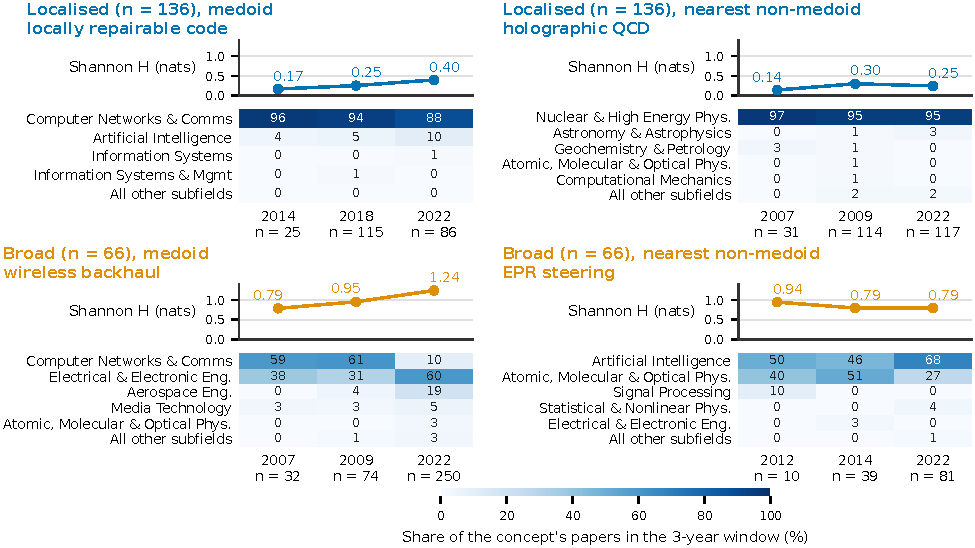
\includegraphics[width=\linewidth,height=0.85\textheight,keepaspectratio]{figures/fig_typology_cases_v0.pdf}
\caption{Representative cases of the $k = 2$ diffusion typology: localised ($n = 136$, top row) and broad-from-the-start ($n = 66$, bottom row). Each row shows the cluster's medoid (left) and the nearest non-medoid concept (right). Localised concepts stay near-monopolised by a single subfield (entropy 0.14--0.40~nats). Broad concepts split across two or more subfields from their first window (entropy 0.79--1.24~nats).}
\label{fig:typology_cases}
\end{figure}

\subsection{Artifact 24: Positioning Dossier (gen\_art\_research\_2)}

\textbf{Novelty verdict: PARTLY ANTICIPATED} (0 ANTICIPATES, 11 PARTLY among 25 graded candidates). No located work measures how host-specific the vocabulary is that a concept is combined with when it enters a new subfield, and relates that, within concepts and across hosts, to later uptake by the host's own newcomers.

Key correction: Cheng et al.\ 2023 measure global embeddedness of new ideas (outcome is yearly article COUNT, not binary ``core'' status). The margin held by this study is: host-specific context at entry, concept fixed effects across hosts, author-disjoint newcomer outcome, sealed-fold confirmation, and MeSH replication.

\subsection{Artifact 25: Paper Figures (gen\_art\_evaluation\_9)}

\begin{table}[!htbp]
\centering
\caption{Figure inventory and production checks (Iteration~5, gen\_art\_evaluation\_9).}
\label{tab:figures}
\begin{tabular}{clccr}
\toprule
Figure & Description & PDF & PNG & Values checked \\
\midrule
F1 & Method flow & Yes & Yes & 39 exact \\
F2 & D2 forest plot & Yes & Yes & 123 exact, 1 derived \\
F3 & Mechanism panel & Yes & Yes & 162 exact, 1 derived \\
F4 & RQ1 held-out & Yes & Yes & 94 exact, 8 derived \\
F5 & Occupancy-rooting & Yes & Yes & 67 exact \\
F6 & Case studies & Yes & Yes & 425 exact \\
F6b & Case ego-networks & Yes & Yes & 8 images \\
F7 & Self-test & Yes & Yes & 0 (schematic) \\
\bottomrule
\end{tabular}
\end{table}

All 8 figures pass production checks. Total: 957 values checked, 0 failures, value fidelity 1.0.

\subsection{Dead Ends and Negative Results (Iteration~5)}

\begin{enumerate}
\item \textbf{EST\_bin null on held-out.} The binary establishment threshold shows $+2.54$~pp per SD with $p = 0.16$.
\item \textbf{Intensive margin is conditional, not causal.}
\item \textbf{Field boundary not detected.} Wald $p = 0.638$.
\item \textbf{MeSH retention slightly lower in host-specificity test.} 12.4\% of $A_{\text{cont}}$ effect absorbed by field breadth on MeSH.
\item \textbf{Audit reveals 292 MISSING\_IN\_REPORT rows.}
\item \textbf{Table~18 self-test: 4 of 11 claims NOT DONE.}
\item \textbf{Seeded-perturbation recall 0.60.}
\end{enumerate}

%% ============================================================
\section{Run Ledger}
\label{sec:ledger}
%% ============================================================

{\small
\begin{longtable}{L{4cm}llcr}
\caption{Run ledger: all artifacts across iterations.} \label{tab:ledger} \\
\toprule
Artifact & Type & Status & Iter. & OA credits \\
\midrule
\endfirsthead
\toprule
Artifact & Type & Status & Iter. & OA credits \\
\midrule
\endhead
gen\_art\_dataset\_1 (pool) & dataset & succeeded & 1 & 2,566 \\
gen\_art\_dataset\_2 (background) & dataset & failed (timeout) & 1 & 1,952 \\
gen\_art\_dataset\_3 (MeSH) & dataset & succeeded & 1 & 1,784 \\
gen\_art\_dataset\_4 (grounding) & dataset & succeeded & 1 & 1,847 \\
gen\_art\_research\_1 (dossier) & research & succeeded & 1 & -- \\
gen\_art\_dataset\_5 (hydrated) & dataset & succeeded & 2 & 7,237 \\
gen\_art\_experiment\_1 (grounding) & experiment & succeeded & 2 & -- \\
gen\_art\_experiment\_2 (viability) & experiment & succeeded & 2 & -- \\
gen\_art\_experiment\_3 (emergence, main) & experiment & succeeded & 2 & -- \\
gen\_art\_experiment\_4 (emergence, MeSH) & experiment & succeeded & 2 & -- \\
gen\_art\_evaluation\_1 (audit) & evaluation & succeeded & 3 & -- \\
gen\_art\_experiment\_5 (emergence deepen) & experiment & succeeded & 3 & -- \\
gen\_art\_experiment\_6 (breadth prediction) & experiment & succeeded & 3 & -- \\
gen\_art\_experiment\_7 (host-entry grafting) & experiment & succeeded & 3 & -- \\
gen\_art\_experiment\_8 (descriptive diffusion) & experiment & succeeded & 3 & -- \\
gen\_art\_evaluation\_2 (grafting held-out) & evaluation & succeeded & 4 & -- \\
gen\_art\_experiment\_9 (MeSH replication) & experiment & succeeded & 4 & -- \\
gen\_art\_evaluation\_3 (closure held-out) & evaluation & succeeded & 4 & -- \\
gen\_art\_evaluation\_4 (descriptive held-out) & evaluation & succeeded & 4 & -- \\
gen\_art\_evaluation\_5 (adopter mechanism) & evaluation & succeeded & 4 & -- \\
gen\_art\_evaluation\_6 (margin decomposition) & evaluation & succeeded & 5 & -- \\
gen\_art\_evaluation\_7 (host-specificity) & evaluation & succeeded & 5 & -- \\
gen\_art\_evaluation\_8 (full audit) & evaluation & succeeded & 5 & -- \\
gen\_art\_research\_2 (positioning dossier) & research & succeeded & 5 & -- \\
gen\_art\_evaluation\_9 (paper figures) & evaluation & succeeded & 5 & -- \\
\bottomrule
\end{longtable}
}

%% ============================================================
\section{Coverage Against the Original Request}
\label{sec:coverage}
%% ============================================================

\begin{table}[!htbp]
\centering
\caption{Final coverage against the original request.}
\label{tab:coverage}
{\small
\begin{tabular}{clL{6cm}}
\toprule
\# & Activity & Status and caveats \\
\midrule
1 & Prepare and semantically ground dataset & Done. Grounding covers focal concepts only; co-word network uses ${\sim}$27k legacy OpenAlex nodes. \\
2 & Construct evolving knowledge network & Done. Legacy-concept nodes; variant normalisation minimal. \\
3 & RQ1: temporal network analysis & Done. R1\_DEAD on primary; persistent-neighbour confirmed. \\
4 & RQ2: cross-disciplinary diffusion & Done. Grafting confirmed + MeSH replicated + K1/K2/K3 decomposition. Primary spec underpowered; Physics null within sampling variation; EST\_bin null on held-out; intensive margin conditional. \\
5 & Identify recurring trajectories & Done. $k = 2$ replicates on held-out and MeSH. Finer typologies unstable; 3-channel adds nothing beyond entropy. \\
6 & Validate with representative cases & Done. Four medoid cases with ego-network visualisations and alluvial paths. \\
\bottomrule
\end{tabular}
}
\end{table}

%% ============================================================
\section{What the Run Learned Overall and What Is Still Open}
\label{sec:conclusions}
%% ============================================================

\subsection{Confirmed Findings}

\textbf{Host-entry grafting predicts durable integration.} When a concept enters a new host subfield, the share of its initial co-occurrence partners that are native to that host predicts subsequent uptake by newcomer authors. This holds on the held-out fold (co-primary IRR/SD 1.19 [1.06, 1.33], $p = 0.004$) and replicates on the independent MeSH population (IRR/SD 1.23 [1.12, 1.36], Holm $p < 0.001$). The IVW pooled estimate is 1.26 [1.17, 1.36] with $I^2 = 0$. Co-transfer (arriving with origin companions) is null across all folds and populations.

The effect operates through both the extensive margin (IVW $+6.43$ pp/SD [4.76, 8.11]) and the intensive margin (IVW IRR/SD 1.183 [1.104, 1.267]), is host-specific rather than reflecting general accessibility (IVW retention 0.969 after generality controls; Balassa-index $A_{\text{lift}}$ IVW IRR/SD 1.34 [1.23, 1.46]), and does not vary by origin field (Wald $p = 0.638$).

\textbf{Persistent-neighbour closure is confirmed.} Among stable top-20 associates, emerging concepts show lower triadic closure before onset (held-out $S = -1.073$, Holm $p = 0.015$). Burt constraint is positive on both folds, ruling out a simple brokerage interpretation.

\textbf{Expansion precedes diffusion.} In 25 of 26 pooled main-arm dual-onset concepts, network expansion precedes disciplinary diffusion.

\subsection{Dead Findings}

\begin{itemize}
\item \textbf{R1\_DEAD:} The general closure deficit did not survive held-out confirmation on the primary operationalisation (Holm $p = 0.147$).
\item \textbf{Source-sink viability:} Blocked by Gate~A failure (within-host traced share 0.17).
\item \textbf{Breadth prediction:} Openness does not predict where concepts travel beyond growth baselines.
\item \textbf{Closure-anchoring link:} Null. The two findings (closure and grafting) are independent.
\item \textbf{Co-transfer:} Null across all specifications and populations.
\end{itemize}

\subsection{Adopter-Level Mechanism}

Adopters are 3.1 times more likely than matched non-adopters to have prior exposure to the concept's entry partners (OR 3.09 [2.32, 4.28]), with enrichment strongest for origin-vocabulary (FOREIGN) partners (OR 2.88). This is consistent with absorptive capacity or topical proximity. The vocabulary-class gradient (FOREIGN $>$ NATIVE) runs opposite to the entry-level grafting finding, indicating that the two levels operate through different channels: at the entry level, host-native partners lower the barrier for newcomers who lack origin expertise; at the adopter level, those who adopt tend to have origin expertise already.

\subsection{What Is Still Open}

\begin{enumerate}
\item \textbf{Generalisation beyond physics/CS/biomedicine.} The population is dominated by arXiv-sourced concepts. Social sciences and humanities are untested.
\item \textbf{Binary establishment threshold.} EST\_bin is null on the held-out fold ($p = 0.165$). The effect predicts uptake initiation, not strict establishment.
\item \textbf{Primary specification.} The fully saturated primary specification remains inconclusive on the held-out fold (IRR/SD 0.98, $G = 30$).
\item \textbf{Single-paper caveat.} 87\% of co-primary events are single-paper entries. On the held-out fold, the single-paper interaction ratio is 0.80 ($p = 0.004$).
\item \textbf{Causal identification.} The study design is observational. Host-nativeness of entry partners is not randomly assigned.
\item \textbf{Finer diffusion typologies.} Only $k = 2$ is stable; finer typologies are unstable.
\item \textbf{The absorptive-capacity vs topical-proximity distinction} at the adopter level cannot be resolved with this design.
\end{enumerate}

\subsection{Pre-Registration Integrity}

All pre-registered specifications were frozen and hashed before outcome data were inspected. Fourteen specifications were hashed in total, covering the concept frame, viability rules, test population, turnover pre-check, emergence deepen, host-entry grafting, descriptive diffusion held-out, held-out confirmation, grafting held-out, discriminating tests, MeSH replication, closure-anchoring link, and the K1/K2/K3 decomposition. Hash digests are recorded in the run's artifact metadata and can be verified against the original specification files.

\end{document}
